Gyrotron is based on the phenomenon termed as ECR (Electron Cyclotron Resonance) which is instability caused to relativistic rotating electrons in a constant magnetic field, with an electric field of the electromagnetic wave which causes electrons to oscillate and radiate electromagentic waves, hence classifying this device as a CEM (Classical Electron Maser).\\

A free electron moves along a toroidal trajectory when subject to a uniform static electric and magnetic field. The electron gun in the gyrotron generates a hollow beam of electrons, consisting of smaller beams called beamlets. Each electron in every helical beamlet is subjected to an alternating electric field.\\

\begin{figure}
\centering
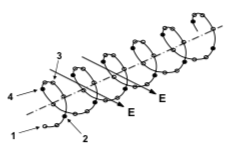
\includegraphics{./images/beamlet}
\caption{A beamlet travelling along the tube in the electric field}
\label{fig:beamlet}
\end{figure}

Considering one beamlet ( see figure \ref{ fig:beamlet } ), the electrons in position number 1 and 3 along the helical beam encounter deceleration and acceleration respectively, as each of them are moving in the direction and opposite to the direction of  electric field at that instant respectively. Electrons in positions 2 and 4 are moving perpendicular to the field so their mass is not being affected. This varying effect of electric field on various positions on the helix causes the electrons to form bunched electrons moving along the direction of electric field, energy is lost by the electron bunch indicating transfer of energy from the electrons to the electric field on each half-cycle of the alternating field.\\

The combination of many beamlets undergoing loss of energy every half-cycle causes amplification of the field when all of them synchronize.